\section{Introduction}
The codebases of software products have increased yearly, now spanning to millions making it hard to grasp the knowledge of the projects \cite{mcmillan2013portfolio}. All this
code needs to be rapidly developed and also maintained. As the amount of code is tremendous, it is an easy opportunity for bugs to slip in.

There are multiple tools that can help with this issue. Most of the time, working professionals rely on static code analyzers such as the ones found in IntelliJ IDEA\footnote{\url{https://www.jetbrains.com/idea/}}. However, these contain a lot of false positives or miss the bugs (such as most off-by-one errors) which make the developers ignore the results of the tools \cite{goseva2015capability}. Recently, a lot of Artificial Intelligence solutions have emerged which help with the issue \cite{alon2019code2vec, pradel2018deepbugs, allamanis2017learning, vasic2019neural}. Although they are not a panacea, they provide enhanced aid to developers in different steps of developing processes, highlighting the potentially faulty code before it gets into production.

One particular solution by Alon et al., the Code2Vec model \cite{alon2019code2vec} (see Section \ref{sec:relevant_literature} for description), delivers state-of-the-art performance on method naming. The authors do not test the model on other tasks, however, they theorize that it should also yield good performance. 

In this work, we use the Code2Vec deep learning model and replace the layer for method naming with a binary classification layer. The aim is to repurpose the model for detecting off-by-one logic errors found in boundary conditions (see Section \ref{sec:data}). Our intuition is that the change in the Abstract Syntax Tree (AST) weights upon introducing a bug as seen in Figure \ref{fig:AST_exclamation} is learnable by our model. Hence the system should be able to learn to identify off-by-one bugs.

The main contributions of this paper are.
\begin{itemize}
    \item Replicating work done by authors of Alon et al. \cite{alon2019code2vec}
    \item Quantitative and qualitative evaluation of a Code2Vec's performance on a task other than method naming.
\end{itemize}

The paper is divided into the following sections. In Section \ref{sec:relevant_literature} the relevant literature used to create this paper is discussed, in Section \ref{sec:data} the data origins and preprocessing is explained, in Section \ref{sec:model} the architecture and training of the model are discussed. Finally, in Section \ref{sec:evaluation}, the model is evaluated which is followed by some reflections regarding our work in Section \ref{sec:discussion} and a conclusion in Section \ref{sec:conclusion}.

\begin{figure*} 
  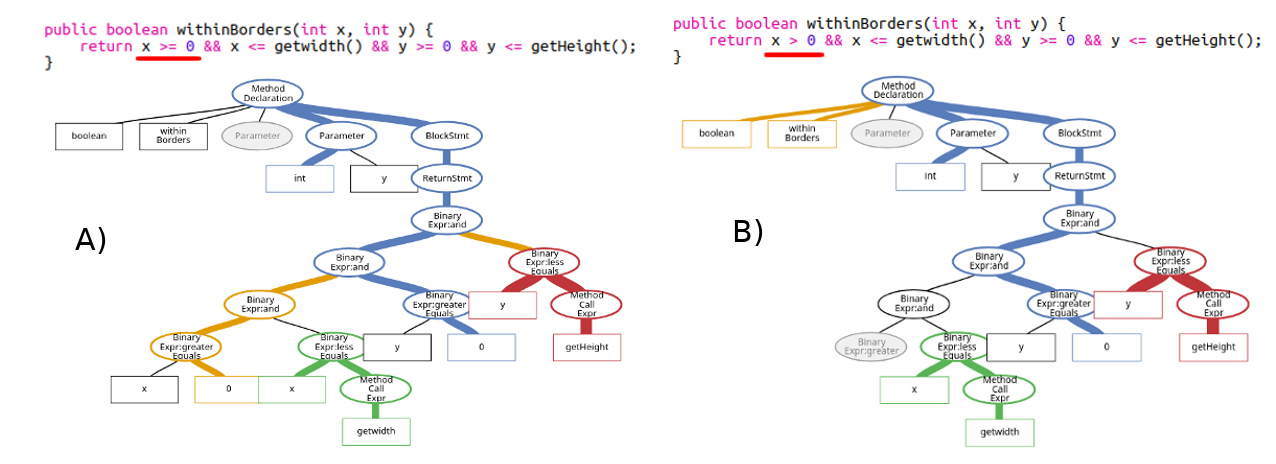
\includegraphics[width=\textwidth,height=8cm]{figures/AST_example.png}
  \caption[]{Example change of AST weights after introducing bug using Code2Vec web interface\protect\footnotemark} (Option \textit{A} being correct and \textit{B} incorrect code)
  \label{fig:AST_exclamation}
\end{figure*}

\footnotetext{\url{https://code2vec.org/}}